\documentclass{article}
\usepackage[utf8]{inputenc}
\usepackage{makeidx,amsmath,amssymb,exscale,multicol,graphics,verbatim,float,subfig,amsthm,url}
\usepackage[all,knot,poly]{xy}
% \usepackage[dvips]{color}
\usepackage{epsfig}
\usepackage{afterpage,array}
\usepackage{setspace}
\usepackage{booktabs}

% Diagrams
\usepackage{mdframed}

% Tikz
\usepackage{tikz}
% \usetikzlibrary{graphdrawing}
\usetikzlibrary{graphs}
% \usegdlibrary{trees}
\usetikzlibrary{calc}

% Todo notesibtex tod
\usepackage{xargs}
\usepackage{xcolor}
\usepackage[colorinlistoftodos,prependcaption,textsize=tiny]{todonotes}
%
\definecolor{MidnightBlue}{rgb}{0.1, 0.1, 0.44}
\definecolor{CornflowerBlue}{rgb}{0.39, 0.58, 0.93}
\definecolor{shadecolor}{rgb}{0.8,0.8,0.8}
\definecolor{Black}{rgb}{0.0, 0.0, 0.0}
\definecolor{BrickRed}{rgb}{0.8, 0.25, 0.33}

\usepackage{hyperref}
\makeindex
\hypersetup{backref,
  pdftitle=The GNUnet System,
  pdfauthor=Christian Grothoff,
  pdfkeywords=peer-to-peer security privacy decentralisation dht networks,
  pdfsubject=Network security,
  colorlinks=false}

\newcommand{\rr}{$R^5N$}
\newtheorem{newdef}{Definition}
\newtheorem{definition}{Definition}
\newtheorem{lemma}{Lemma}
\newtheorem{theorem}{Theorem}
\newtheorem{corollary}[theorem]{Corollary}


\title{Counting common contacts to improve trust on first use}
\author{Jeffrey Burdges \and Christian Grothoff}

\begin{document}
\maketitle


\def\Z{\mathbb{Z}}

\newcommand*\set[1]{\{ #1 \}} % in text, we don't want {} to grow
\newcommand*\Set[1]{\left\{ #1 \right\}}
\newcommand*\setst[2]{\{ #1 | #2 \}}
\newcommand*\Setst[2]%
        {\left\{\,#1\vphantom{#2} \;\right|\left. #2 \vphantom{#1}\,\right\}}

\newcommand*\List[1]{\left[ #1 \right]}  % cute abbreviations
\newcommand*\listst[2]{[ #1 | #2 ]}
\newcommand*\Listst[2]%
        {\left[\,#1\vphantom{#2} \;\right|\left. #2 \vphantom{#1}\,\right]}

\def\Alice{{\textrm{Alice}}}
\def\Bob{{\textrm{Bob}}}

\def\mathcomma{,}
\def\mathperiod{.}


In~\cite{p4t} we proposed a protocol for private set intersection
cardinality with signatures.  This protocol allows two participants
to securely compute the set intersection cardinality of two sets,
where one of the participants has his set signed by the members
in the set.

We envision using the protocol for privacy-preserving detection of
abusive behavior in OSNs, where a large overlap between Alice's
subscriptions and Bob's subscribers is an indicator of
the benign nature of Bob.

One also could envision the protocol used to assess the validity of
public keys for an entity in a privacy-enhanced variant of the
Web-of-trust, where the users sign each other's keys but do not expose
the resulting social graph to the world.

We will now briefly sketch the new protocol (which is yet to be
implemented).

\subsubsection{The Boneh-Lynn-Shacham (BLS) signature scheme}

We first outline the BLS signature scheme~\cite{BLS-SigWeilPairing},
which begins with a Gap co-Diffie-Hellman group pair $(G_1, G_2)$ of order $p$
with an efficiently-computable bilinear map $e\colon G_1\times G_2 \to G_T$,
 a generator $g_2$ of $G_2$,
% $\phi$ an efficiently computable isomorphism from $G_2$ to $G_1$,
 and a cryptographic hash function $H_1 : \{0,1\}^* \to G_1$.

In the BLS scheme, a private key consists of a scalar $c \in \Z/p\Z$,
while the corresponding public key is $C := g_2^c$, and a signature on
a message $m$ by $C$ is $\sigma := H_1(m)^c$.

A signature $\sigma$ is verified by checking that $e(H(m),C) =
e(\sigma,g_2)$.  If $\sigma = H(m)^c$ then this holds by bilinearity
of $e$.

\subsubsection{Our protocol}

We define $Z' := \setst{ h(x) }{ x \in Z }$
 whenever $Z$ is some set under discussion, and assume a fixed
system security parameter $\kappa \ge 1$ has been agreed upon.
Each participant is identified by a public key pair $C = g_2^c$
for the BLS signature scheme.  Each participant $A$ has a subscriber
list $L_A$ consisting of tuples $(C,\sigma_{A,C})$ where
$\sigma_{A,C} := H_1(A||\texttt{date})^c$ is a BLS signature affirming
that $C = g_2^c$ was subscribed to $A$ until some expiration
$\texttt{date}$, the specifics of which depend on the application.
We envision these signatures being provided in advance so that Bob's
subscribers need not be online when running the protocol.

Suppose Alice wishes to know $n := |L_\Alice \cap L_\Bob|$.
First, she generates an ephemeral private scalar $x_A \in
\Z/p\Z$ and sends Bob
\begin{equation}
{\cal X}_\Alice := \texttt{sort}
  \Listst{ C^{x_A} }{ (C, \sigma_{A,C}) \in L_\Alice }
  \mathperiod
\end{equation}
Second, Bob picks ephemeral private scalars
 $t_{\Bob,j} \in \Z/p\Z$ for $j \in 1,\ldots,\kappa$ and
 computes
\begin{align}
  {\cal X}_{\Bob,j} :&= \texttt{sort}
  \Listst{ C^{t_{\Bob,j}} }{ (C, \sigma_{B,C}) \in L_\Bob }  \\
  {\cal Y}_{\Bob,j} :&= \texttt{sort}
  \Listst{ \overline{C}^{t_{\Bob,j}}}{ \overline{C} \in {\cal X}_\Alice }
  \mathperiod
\end{align}
For $j \in 1,\ldots,\kappa$ and $(C,\cdot) \in L_\Bob$,
Bob picks more ephemeral private scalars $s_{j,C} \in \Z/p\Z$ and
computes $S_{j,C} := g_2^{s_{j,C}}$ and
 $\sigma_{B,S_{j,C}} := H_1(B||\texttt{date})^{s_{j,C}}$.
Let $\pi$ denote the permutation applied by the $\texttt{sort}$ for ${\cal X}_{\Bob,j}$.
Bob also computes
\begin{align}
  {\cal U}_{\Bob,j} :&= \pi
  \Listst{ C^{t_{\Bob,j}} S_{j,C} }{ (C, \sigma_{B,C}) \in L_\Bob }  \\
  {\cal V}_{\Bob,j} :&= \pi
  \Listst{ \sigma_{B,C}^{t_{\Bob,j}} \sigma_{B,S_C} }{ (C, \sigma_{B,C}) \in L_\Bob }
  \mathperiod
\end{align}
He then sends to Alice the commitments
 ${\cal U}'_{\Bob,i}$, % Needs ' or else adversary can find S_{j,C}
 ${\cal Y}'_{\Bob,i}$, and
 ${\cal V}'_{\Bob,i}$ for $i \in 1,\ldots,\kappa$.

Third, Alice picks a non-empty random $J \subseteq \{1,\ldots,\kappa\}$
 and sends $J$ to Bob.

Fourth, Bob sends
 Alice his scalar $t_{\Bob,j}$ along with
 ${\cal U}_{\Bob,j}$ and ${\cal V}_{\Bob,j}$ for $j \notin J$,
as well as
 ${\cal X}_{\Bob,j}$ and his scalars
 $\pi [ s_{j,C} | (C, \sigma_{B,C}) \in L_\Bob ]$ for $j \in J$.

Fifth, Alice verifies Bob's commitments :
For $j \notin J$, Alice checks the $t_{\Bob,j}$ matches the
 commitment ${\cal Y}'_{\Bob,j}$ by computing ${\cal Y}_{\Bob,j}$ herself.
Also for $j \notin J$, Alice checks that ${\cal V}_{\Bob,j}$
 matches the ${\cal V}'_{\Bob,j}$ and verifies the signatures in
 ${\cal V}_{\Bob,j}$ using ${\cal U}_{\Bob,j}$ as public keys.
These signatures validate because we employ the BLS pairing based
signature scheme where:
\begin{align*}
 e( H_1(B||\texttt{date}), C^{t_{\Bob,j}} S_{j,C} )
 &= e (H_1(B||\texttt{date}), g_2^{t_{\Bob,j} c + s_{j,C}}) \\
 &= e( H_1(B||\texttt{date}), g_2 )^{t_{\Bob,j} c + s_{j,C}} \\
 &= e( H_1(B||\texttt{date})^{t_{\Bob,j}c + s_{j,C}}, g_2 ) \\
 &= e( H_1(B||\texttt{date})^{t_{\Bob,j}c} H_1(B||\texttt{date})^{s_{j,C}}, g_2 ) \\
 &= e( \sigma_{B,C}^{t_{\Bob,j}} \sigma_{B,S_C}, g_2 )
\end{align*}
% TODO : Should we distribute across the group operation to keep the
% original signature in tact here, like we had before?
For $j \in J$, Alice verifies ${\cal U}'_{\Bob,j}$ by computing it
 herself from ${\cal X}_{\Bob,j}$ and the $s_{j,C}$.

For $j\in J$, Alice computes
\begin{equation}
  {\cal Y}_{\Alice,j} :=
  \Setst{ \hat{C}^{x_A}}{ \hat{C} \in {\cal X}_{\Bob,j} }
  \mathperiod
\end{equation}
Finally, she obtains the result from
$|{\cal Y}'_{\Alice,j} \cap {\cal Y}'_{\Bob,j}| = n$ for $j \in J$,
checking that these values agree for all $j \in J$.

An attack on this blinded signature scheme translates into an attack
on the underlying BLS signature scheme.  If Bob tries to manipulate to
increase the overlap, the cut-and-choose part detects this with
probability $1:2^\kappa$.


\section{Protocol security}

We briefly give an intuition behind the design of our protocols
in Section~\ref{5.7} and Section~\ref{5.8} for computing
the number of common subscribers and subscriptions respectively.

As above, suppose Alice wants to know the overlap of subscriptions or
subscribers she has with Bob, namely $n := |{\cal L}_A \cap {\cal L}_B|$.
Each user has a private key $c_i$ and
the corresponding public key is $C_i := g^{c_i}$ where
 $g$ is the group generator.
Let ${\cal L}_A$ be the set of public keys representing
Alice's subscriptions and ${\cal L}_B$ be the set of keys representing
Bob's subscriptions.

We first consider a simple straw-man protocol:
Alice begins by creating an ephemeral private scalar $t_A \in \Z/p\Z$
and sending Bob her blinded friends lists
\begin{equation}
  {\cal X}_A := % \texttt{sort}
  \Listst{ C^{t_A} }{ C \in {\cal L}_A }
  \mathperiod
\end{equation}
Bob replies by creating an ephemeral private scalar $t_B \in \Z/p\Z$
and sending Alice his blinded friends lists and her list reblinded
\begin{align}
  {\cal X}_B :&= % \texttt{sort}
  \Listst{ C^{t_B} }{ C \in {\cal L}_B }  \\
  {\cal Y}_B :&= % \texttt{sort}
  \Listst{ \overline{C}^{t_B} }{ \overline{C} \in {\cal X}_A }
  \mathperiod
\end{align}
Alice computes
\begin{equation}
  {\cal Y}_A :=
  \Setst{ \hat{C}^{t_A}}{ \hat{C} \in {\cal X}_B }
  \mathperiod
\end{equation}
Finally, Alice gets $|{\cal Y}_A \cap {\cal Y}_B| = n$.
% Alice may send ${\cal Y}_A$ to Bob if he wishes to compute $n$ too.

We address several types of attacks on this scheme
 in Section~\ref{ssec:protocol1}:

First, we assume Alice or Bob can place sock puppet accounts among
the other's subscriptions or subscribers lists.
If say Bob inserts $C^k$ in Alice's list ${\cal L}_A$, then
he can identify if $C$ lies in ${\cal X}_A$. % because
\begin{equation}
   C \in {\cal L}_A \iff
   {\cal X}_A \cap
   \Setst{ \overline{C}^k }{ \overline{C} \in {\cal X}_A}
   \neq \emptyset
  \mathperiod
\end{equation}
We block this attack this by requiring a signature from contacts
joining subscription or subscriber lists.  Alice and Bob can still
place sock puppets, but only ones for whom they know the private
key, so then this attack no longer yields information.

Now, suppose Bob creates sock puppets accounts in pairs $S_i$ and $S_i^k$ where
Bob knows only $k$.  Then he also knows
\begin{equation}
   \{ S_i^k \} =
   {\cal X}_A \cap
   \Setst{ \overline{C}^k }{ \overline{C} \in {\cal X}_A }
  \mathperiod
\end{equation}
As he knows these elements' locations in ${\cal X}_A$,
he can deduce the number of Alice's contacts $C$ with
$S_i < C < S_{i+1}$ for all $i$ where $<$ denotes whatever
ordering Alice's original contact list ${\cal L}_A$ possessed.
This would allow Bob to obtain information
 about Alice's contact list.
Alice defeats this by sorting her list after blinding, which
produces a random ordering, by our discrete logarithm assumptions.
For the same reasons, Bob must sort ${\cal X}_B$ as well.
%, even if he does not care to learn $n$.

Third, Alice wishes to examine Bob's relationship with some real
contact $C$ that she may or may not not know, but for which she
lacks the private key.  Alice picks a secret marker scalar $k$
and places $C$ along with a a sock puppet $C^k$ into her own list.
If Alice is given ${\cal Y}_B$, then she could identify the pair
of elements  $\overline{C}, \overline{C}^k \in {\cal Y}_B$
 as above, and then check if $\overline{C} \in {\cal Y}_A$
to test if $C \in {\cal L}_B$.  We therefore only send
the hashed ${\cal Y}'_B$, never ${\cal Y}_B$ itself.

% Alice could embed key splittings of
% Bob sorts ${\cal Y}_B$ because A

Forth, suppose Bob correctly guesses the $C$ corresponding to
 any $\overline{C} = C^{t_A}$ from ${\cal X}_A$, then
Bob can choose $K \subset \Z/p\Z$ and send fakes using
 ${\cal X} = \listst{ C^k }{ k \in K } \cup \{ \cdots \}$ and
 ${\cal Y} = \listst{ \overline{C}^k }{ k \in K } \cup \{ \cdots \}$,
so that Alice computes $n = |K|$.
%Alice can do the same to Bob if Bob wishes to know $n$ too.
To defend against successful guessing,
Alice and Bob can pad their lists if they are short.
At first blush, we might ask if such attacks could be detected using
padding with tag contacts similar to the first attack, but
our restriction from sending ${\cal Y}_B$ prohibits this.

Instead, we employ a cut and choose protocol to reduce this
change of guessing safely to the desired level.
Presumably the cut and choose protocol is rather costly, but
not that it needs to be run very often.  In addition, attacks that
merely falsify $n$ are not particularly valuable to the adversary, so
they do not require a particularly high security margin for defense.

We encounter a new form of attack in Section~\ref{ssec:protocol1}
due to the use of pairing based cryptography, where
there is no decisional Diffie-Hellman assumption because
$e(g^a,g^b) = e(g^{ab},g)$.  In pairing based cryptography, only the
weaker computational Diffie-Hellman assumption remains tenable.
It follows that, if Alice knows both $\sigma$ and
 $\sigma^{t_A}$ for some $\sigma$, such as our BLS signatures,
then she can compute $e(\sigma,C^t) = e(\sigma^t,C')$ as
 $C'$ runs over all known contacts,
thereby revealing Bob's contact list.

We avoid this by integrating the signature verification with our
cut and choose protocol using additional additive blinding factors
$S_{j,C} := g_2^{s_{j,C}}$.
As an exercise, one might replace these $|{\cal L}_B|$ additive
blinding operations with two multiplicative blinding scalars.
\begin{align*}
e( H_1(B||\texttt{date}), C^{t_{B,j} u_j v_j} )
 &= e( H_1(B||\texttt{date}), g_2 )^{t_{B,j} c u_j v_j} \\
 &= e( \sigma_{B,C}^{t_{B,j} u_j}, g_2^{v_j} )
\end{align*}
We fear this two scalar approach requires more careful security
arguments however.
After natural optimizations, it seemingly fails to reduce either
computation or bandwidth too.

% TODO : additive seems off, group operation perhaps?
% TODO : Picture of chain of revelations?

In a similar vein, we must avoid symmetric pairings because otherwise
an adversary could say fix $X,Y \in {\cal X}_A$ to test
$e(X,U) = e(V,Y)$ for all $U,V$ is some domain of likely contacts.
% TODO: I found one paper that almost names the opposite of this assumption,
% and discusses it's believability, so we could reference them, but doing so
% well seems like a rabbit hole.

% AGR: complexity
\section{Protocol complexity}
%
This appendix describes the computational complexity and
communication overhead of our protocol. Our protocol
design assumes users can collect public keys, and possibly signatures, at
subscription time; either when they subscribe to someone or when
others subscribe to them. We therefore avoid protocol participants
having to engage into more costly communications during protocol
runtime.
% We have engineered the protocol so that users can collect public
% keys, and possibly signatures, during subscription operations.
% We are not engineers. Neither we have implemented the protocol yet.

Assuming this, such information is already available at such time to protocol
participants, then computing a privacy-preserving set intersection
using our protocol only involves two round trips, or four message
exchanges. This is an important aspect that characterizes the
computational complexity and bandwidth overhead of the protocol.

As described, these steps steps each consume $\mathcal{O}(\kappa \cdot n)$ computation
time and bandwidth where $n$ is the number of contacts, and $\kappa$
is our security paramater, except for choosing $J$ which is constant,
and the initiation step, which consumes only $\mathcal{O}(n)$ computation time
and bandwidth.  We feel this cost is reasonable because $\kappa$ need
not to be chosen to have cryptographic size, as noted above, and the
constant terms hidden by the Big $\mathcal{O}$ notation consists of a few public key
operations. There remains some freedom for optimizing bandwidth usage
during the commitment phase however.

% AGR: we still want to be more detailed about it.
\medskip
\paragraph{Computational complexity}
%
Alice needs to compute the list to send to Bob in
equation~\ref{eq:alice:computes-send:1}. Such operation only incurs
linear cost, which is directly proportional to the number and size of
public keys $C_i\in {\cal L}_A$ involved in the blinding she needs to do
before sending such list to Bob. The cost of this operation is
$\mathcal{O}(pk \cdot setsize)$, whereas $pk$ is the actual size
of the keys being blinded. Likewise, Bob operates the same blinding on his list
${\cal L}_B$ and Alice's blinded list when he receives it, so the cost
for hims is about two times more than for Alice if we both had the
same number of contacts.
% TODO: Shall we consider 64, 128 for public keys cost above?
% TODO: What about the size of the blinding scalar?

% The final computational complexity is, $\mathcal{O}(x)$ for Alice
% and $\mathcal{O}(y)$ for Bob, so in summary $\mathcal{O}(x + y)$.

\medskip
\paragraph{Bandwidth overhead}
%
Now we analyse the bandwidth cost for each party, Alice and Bob.  The
first message exchange by Alice simply involves her blinded list of
contacts.

In the second message exchange, Bob responds with the commitments from
Equations~\ref{eq:bob:sends:1}. Therefore the bandwidth overhead is
presumably higher for him in this round than for Alice in the first.
 % ${\cal Y}'_{B,i} \quad{for \hspace{2mm} i \in 1,\ldots,\kappa}$

 % The final bandwidth overhead or cost is, $\mathcal{O}(x)$ for Alice
 % and $\mathcal{O}(y)$ for Bob, so in summary $\mathcal{O}(x + y)$.

% TODO: Final protocol
\begin{figure}[t]
  \begin{mdframed}
    \centering
    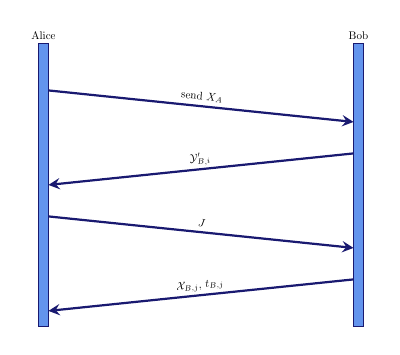
\begin{tikzpicture}[scale = 0.4, transform shape, msglabel/.style
      = { text = Black, yshift = .3cm, sloped, midway }, okmsg/.style
      = { ->, color = MidnightBlue, thick, >=stealth }, rstmsg/.style
      = { ->, color = BrickRed, thick, >=stealth } ]
      \node[draw = MidnightBlue, fill = CornflowerBlue, minimum width
      = .3cm, minimum height = 9cm ] (h1) at (-5, 0) {}; \node[draw =
      MidnightBlue, fill = CornflowerBlue, minimum width = .3cm,
      minimum height = 9cm ] (h2) at (5, 0) {}; \node[above = 0cm of
      h1] {Alice}; \node[above = 0cm of h2] {Bob};

      \path[->, color = MidnightBlue, thick, >=stealth]
      ($(h1.east)+(0,3)$) edge node[text = Black, yshift = .3cm,
      sloped] {send $X_A$} ($(h2.west)+(0,2)$); \path[->, color =
      MidnightBlue, thick, >=stealth] ($(h2.west)+(0,1)$) edge
      node[text = Black, yshift = .3cm,
      sloped]{${\cal Y}'_{B,i}$} ($(h1.east)+(0,0)$);
      \path[->, color = MidnightBlue, thick, >=stealth]
      ($(h1.east)+(0, -1)$) edge node[text = Black, yshift = .3cm,
      sloped] {$J$} ($(h2.west)+(0, -2)$); \path[->, color =
      MidnightBlue, thick, >=stealth] ($(h2.west)+(0,-3)$) edge
      node[text = Black, yshift = .3cm, sloped] {${\cal X}_{B,j}$,
        $t_{B,j}$} ($(h1.east)+(0,-4)$);
    \end{tikzpicture}
    \caption{Protocol message exchange}\label{protocol-full}
  \end{mdframed}
\end{figure}

\bibliographystyle{alpha}
\bibliography{bibliography}

\end{document}
